\section{The Ball-on-Arc Platform}
\label{sec:system}

\begin{figure}[t]
  \centering
  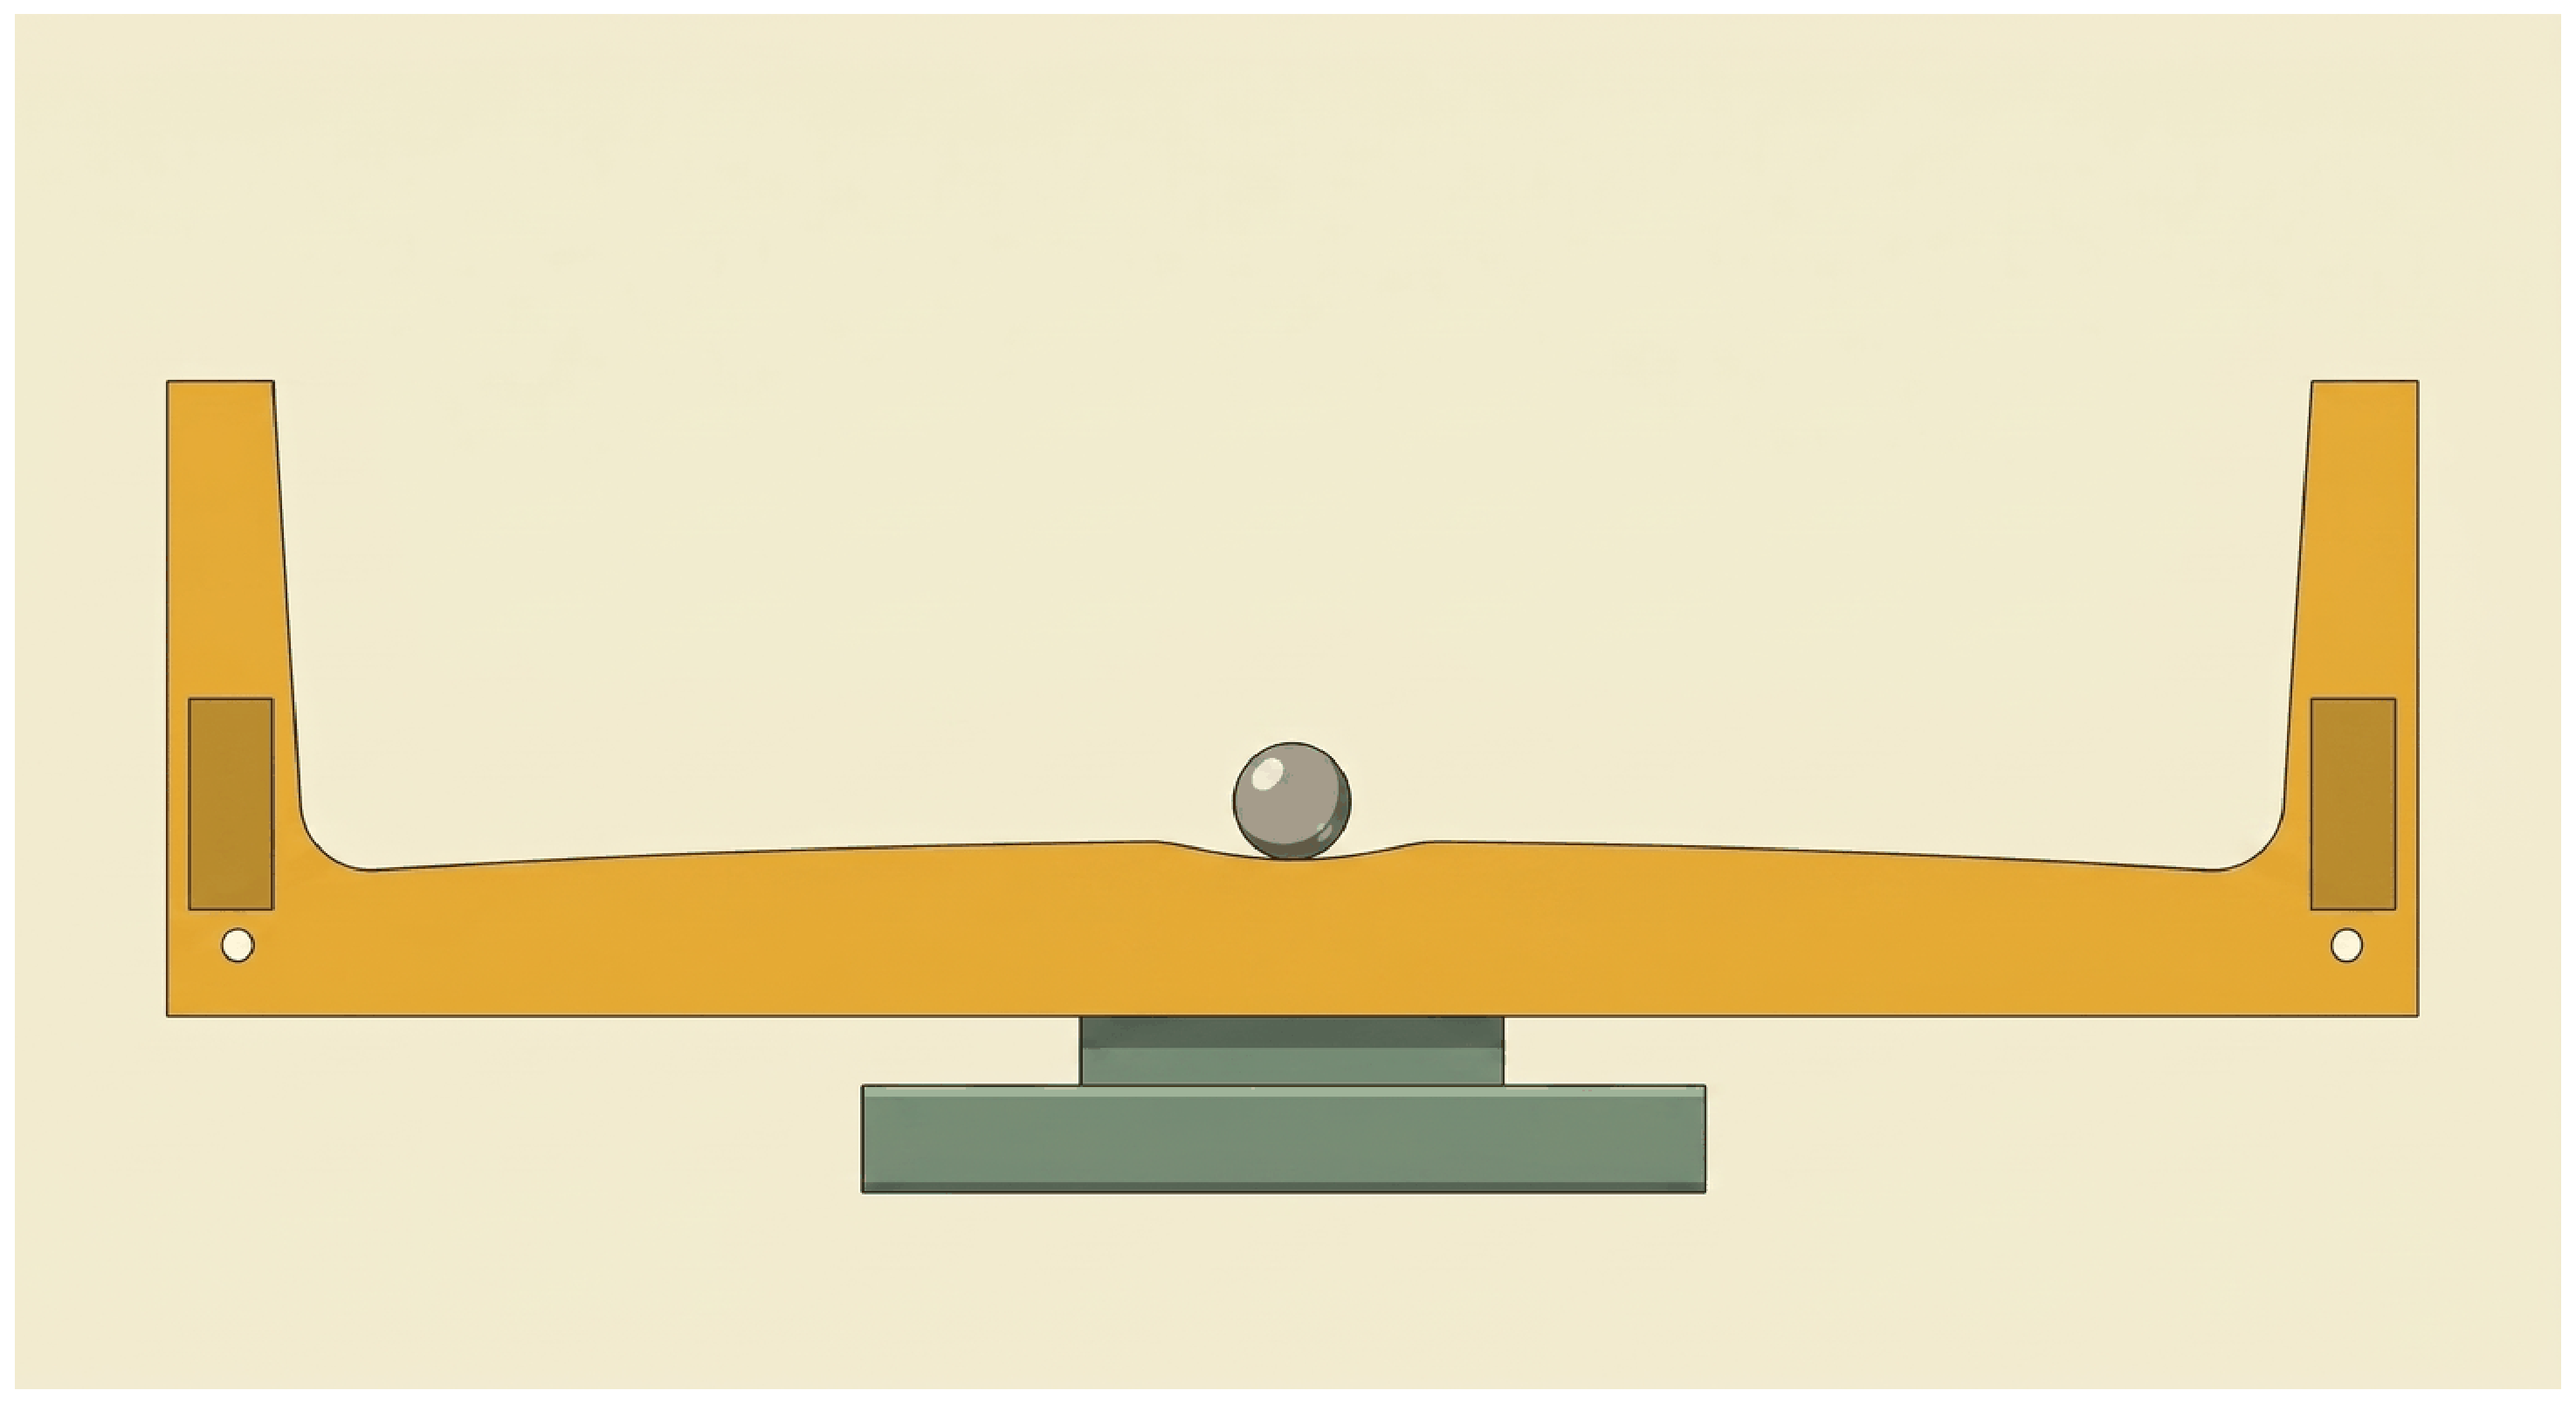
\includegraphics[width=0.9\columnwidth]{figures/ball_on_arc_cart.eps}
  \caption{Cross-section of the cart, a single 3D-printed part whose top
    surface is the arc the ball rolls on. A shallow concave dip at the
    center, where the ball rests, forms a weak but restoring
    gravitational well, so the balance point is locally stable and
    lightly damped. The cart rides the linear actuator below it and
    translates left and right to steer the ball.}
  \label{fig:sketch}
\end{figure}


Our platform is an underactuated ball-on-arc system with a rail-constrained industrial cart and realistic on-board sensing.
The ball is 24\,g and 9\,mm in radius, and the convex arc it rolls on has radius $R = 2.101$\,m with a shallow concave dip at its center (2\,mm deep, Fig.~\ref{fig:sketch}), mounted on a 3D-printed (PLA) cart\footnote{Printable STL models of the cart (with its integrated arc surface) and the mounts are included in the public repository.} riding a motorized linear actuator (Fig.~\ref{fig:setup}).
The dip forms a weak but restoring well, so the balance point is locally stable and lightly damped rather than open-loop unstable like the classical ball-and-beam, and a PD law holds the ball there with no integral term; the difficulty lies in the actuation, the sensing, and the rail.
The cart is moved by a rotary AC servo motor (Beckhoff AM8121) turning a belt-driven linear slide (SMC LEFB32NXS), commanded in velocity through an industrial EtherCAT servo drive (Beckhoff EL7201) under the TwinCAT motion runtime.
The actuator has 1.0\,m of physical stroke; its drive reports positions in axis units, in which the soft-limited workspace spans $\pm$0.78\,m.
All positions and velocities in this article use these axis units (the supplement gives the scaling).

Every controller reads the platform's own signals, with no observer reconstructing state: the ball angle straight from the time-of-flight geometry, its rate as a finite difference of that angle, and the cart's position and velocity from the servo encoder.
Whatever latency and noise the sensors carry therefore reaches each controller unfiltered.%; we quantify both below.

Recovering the ball is a textbook problem, but what makes this platform demanding are four frictions in the hardware:

\noindent\textbf{Underactuation:} The ball cannot be commanded directly, only indirectly by accelerating the cart, so an aggressive correction can destabilize the ball instead of recovering it.

\noindent\textbf{Hard constraints:} The workspace spans 1.56\,m in axis units, about 0.80\,m of the actuator's 1.0\,m stroke.
A controller that ignores the approaching boundary exhausts its maneuvering space on one side, limiting its ability to recover, which makes explicit constraint handling a central design concern on this platform~\cite{brunke2022safe}.

\noindent\textbf{Sensing:} Ball position comes from two VL53L0X Time-of-Flight sensors read alternately; in operation the estimate refreshes every ${\sim}$80--100\,ms (about 10--12\,Hz), well slower than the 50\,ms (20\,Hz) control loop, so the controller acts on ball measurements up to about two control cycles (${\sim}$100\,ms) old while the cart encoder updates synchronously.
Near the arc edge ($|\theta| > 0.071$\,rad), where the ball rolls within a few millimeters of a sensor, the reading enters the VL53L0X near-field \emph{blind zone} and saturates, holding at the boundary until the ball returns.
Even at center the ball-position reading varies about 13\,mm peak-to-peak ($\sigma \approx 3.3$\,mm; the raw per-unit spread is 14--17\,mm), so every controller has to cope with this noise and latency on its own.

\noindent\textbf{Velocity interface:} We command a velocity setpoint (\texttt{MC\_MoveVelocity}) within the axis limit of $\pm$0.9\,m/s, and the drive realizes it through an internal S-curve profiler and the servo's cascaded position, velocity, and current loops.
We model this as a first-order lag ($\tau_v = 0.15$\,s) for control design; the profiler, the inner loops, and the belt compliance do not appear in an open-loop simulator, and contribute to the platform's sim-to-real gap.

The state vector is 4-dimensional: cart position and velocity, ball angle and angular velocity; the control input is a scalar velocity command.
The complete dynamics equations and system parameters are provided in the supplementary material.
